\chapter{Viabilidad}
Este capítulo tiene como objetivo realizar, en base a los objetivos marcados en el capítulo anterior, elaborar un análisis de viabilidad del proyecto, analizando las diferentes tareas que contiene, calculando los correspondientes gastos y sus inherentes riesgos, que pueden afectar, atrasando o incluso impidiendo, la realización del proyecto.

\section{Requisitos funcionales del trabajo}
Los requisitos funcionales de la aplicación (RF a partir de ahora) se elaboran en base a los objetivos descritos y son los siguientes:

\begin{itemize}
	\item Elaborar un estado del arte que analice el campo de la seguridad informática, sus aplicaciones y analice el área del \textit{pentesting}.
	\item Elaborar una aplicación que permita obtener información sobre redes y nodos de la red.
	\item Integrar correctamente herramientas de terceros para lograr que la aplicación resulte lo más escalable posible.
	\item Aplicar principios sobre experiencia de usuario (UX) y sobre el diseño de interfaces gráficas (GUI) para que la aplicación sea lo más sencilla y cómoda de usar.
\end{itemize}


%------------------------------------------------------------------------------


\section{Planificación del tiempo}

\subsection[EDT]{Estructura de Descomposición del Trabajo}
El EDT (Estructura del Desglose del Trabajo o Estructura de Descomposición del Trabajo) es un sistema jerárquico que permite organizar las diferentes tareas de un proyecto. Es una técnica ampliamente usada para gestionar todo tipo de proyectos, especialmente proyectos de software.

A la hora de planificar el tiempo se ha tenido en cuenta un enfoque en dos fases, a las cuales denominaremos Fase 1 y Fase 2. Esto es debido al carácter del proyecto. Por una parte, para elaborar la aplicación anteriormente mencionada, resulta fundamental realizar un estudio sobre el campo del la seguridad informática, más concretamente sobre el área del pentesting, para poder llegar a encontrar las mejores herramientas y técnicas que permitan desarrollarla. Este estudio, bien desglosado y fundamentado, llevará a la obtención de un elaborado estado del arte, que será el principal objetivo de la Fase 1. Además, dicha fase contiene un periodo de aprendizaje y familiarización con diversos conceptos y tecnologías, que también quedarán reflejados.

En la Fase 2, en función de lo aprendido en la Fase 1, se elaborará la aplicación en base a los criterios de implementar diversas utilidades junto a un experiencia de usuario (UX) óptima, que vendrá acompañada de un buen diseño de una interfaz gráfica (GUI).

El EDT completo quedaría tal y como se muestra en la \autoref{fig:edt}.

\begin{landscape}
	
	\begin{figure}[H]
		\centering
		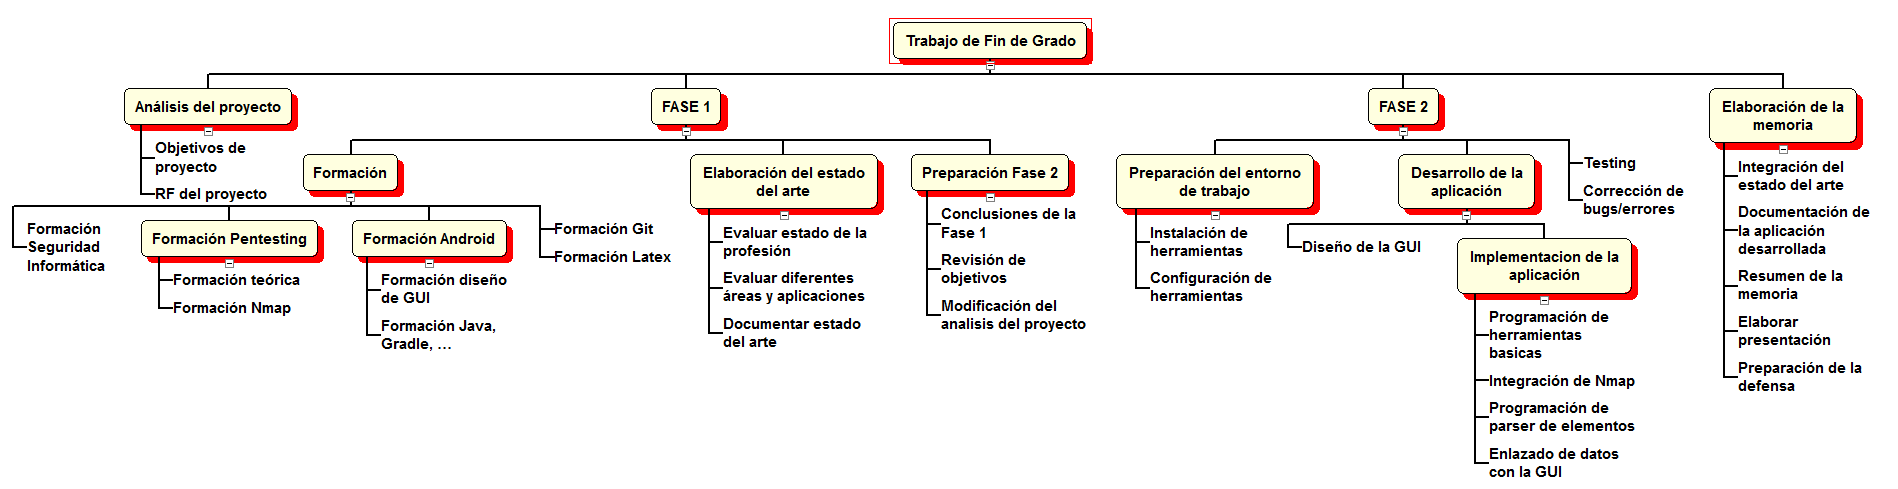
\includegraphics[height=150px]{TFG_EDT}
		\caption{EDT completo}
		\label{fig:edt}
	\end{figure}
	
	\clearpage
	
	\subsubsection{Fase 1}
	El EDT para la Fase 1 quedaría como se muestra en la \autoref{fig:edt1}.
	
	\begin{figure}[H]
		\centering
		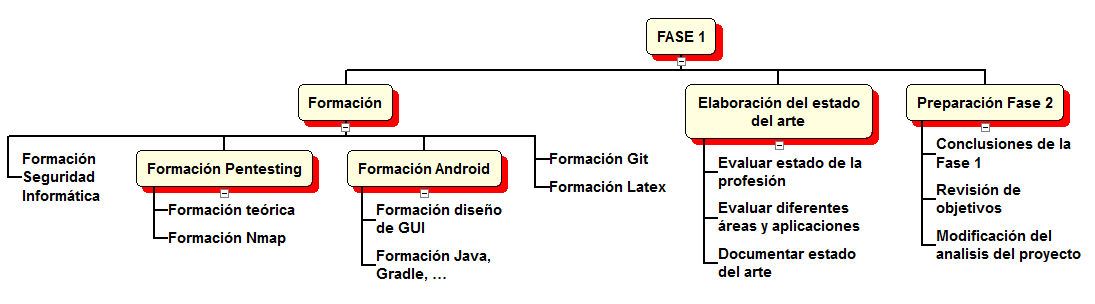
\includegraphics[height=150px]{TFG_EDT_FASE_1}
		\caption{EDT de la Fase 1}
		\label{fig:edt1}
	\end{figure}

\end{landscape}

\subsubsection{Fase 2}
El EDT para la Fase 2 quedaría como se muestra en las \autoref{fig:edt2}.

\begin{figure}[H]
	\centering
	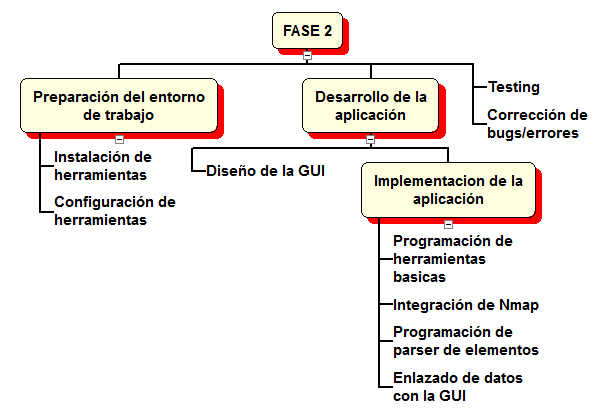
\includegraphics[width=1\textwidth]{TFG_EDT_FASE_2}
	\caption{EDT de la Fase 2}
	\label{fig:edt2}
\end{figure}

\subsection{Agenda del proyecto}
El proyecto se llevará a cabo durante varios meses, comenzando en abril. Se trabajará a media jornada (4 horas) de lunes a viernes, con las siguientes excepciones. Primero, se tendrá en cuenta el calendario de festivos oficiales para aplicar algunas jornadas festivas en cuyos días no se trabajará. Esos días quedan reflejados en la \autoref{table:festivos-oficiales}.

\begin{table}[H]
	\centering
	\begin{tabular}{ |c|c| } 
		\hline
		Fecha & Evento \\
		\hline
		1 de Enero & Año nuevo \\
		6 de Enero & Día de Reyes \\
		19 de Marzo & San José \\
		29 de Marzo & Jueves Santo \\
		30 de Marzo & Viernes Santo \\
		2 de Abril & Lunes de Pascua \\
		28 de Abril & San Prudencio \\
		1 de Mayo & Día del trabajo \\
		25 de Julio & Santiago Apóstol \\
		5 de Agosto & Virgen Blanca \\
		15 de Agosto & Asunción de la Virgen \\
		12 de Octubre & Fiesta Nacional de España \\
		6 de Diciembre & Día de la constitución \\
		8 de Diciembre & Inmaculada Concepción \\
		25 de Diciembre & Navidad \\
		\hline
	\end{tabular}
	\caption{Calendario de días festivos oficial (de Álava)}
	\label{table:festivos-oficiales}
\end{table}

En base a dicho calendario, la fecha estimada de finalización del proyecto es del 16 de enero del 2018.

\subsection{Tareas}
El EDT completo de tareas, al que se añaden la fase inicial de objetivos del proyecto, y toda la fase final de elaboración de la memoria, presentación y la defensa quedaría de la siguiente manera.
\begin{numbered}
	\setcounter{numberedi}{-1} %Para empezar a contar desde 0
	
	\item Análisis del proyecto
	\begin{numbered}
		\item Objetivos del proyecto
		\item RF del proyecto
	\end{numbered}
	
	\item FASE 1
	\begin{numbered}
		
		\item Formación
		\begin{numbered}
			\item Formación seguridad informática
			\item Formación Pentesting
			\begin{numbered}
				\item Formación Teórica
				\item Formación Nmap
			\end{numbered}
			\item Formación Android
			\begin{numbered}
				\item Formación Diseño de GUI
				\item Formación Java, Gradle, ...
			\end{numbered}
			\item Formación Git
			\item Formación \LaTeX
		\end{numbered}
		
		\item Elaboración del estado del arte
		\begin{numbered}
			\item Evaluar estado de la profesión
			\item Evaluar diferentes áreas y aplicaciones
			\item Documentar estado del arte
		\end{numbered}
		
		\item Preparación de la Fase 2
		\begin{numbered}
			\item Conclusiones de la Fase 1
			\item Revisión de objetivos
			\item Modificación del análisis del proyecto
		\end{numbered}
	\end{numbered}
	
	\item FASE 2
	\begin{numbered}
		\item Preparación del entorno de trabajo
		\begin{numbered}
			\item Instalación de herramientas
			\item Configuración de herramientas
		\end{numbered}
		
		\item Desarrollo de la aplicación
		\begin{numbered}
			\item Diseño de la GUI
			\item Implementación de la aplicación
			\begin{numbered}
				\item Programación de herramientas básicas
				\item Integración de Nmap
				\item Programación de parser de elementos
				\item Enlazado de datos con la GUI
			\end{numbered}
			\item Testeo
			\item Corrección de bugs/errores
		\end{numbered}
	\end{numbered}
	
	\item Elaboración de la memoria
	\begin{numbered}
		\item Integración del estado del arte
		\item Documentación de la aplicación desarrollada
		\item Resumen de la memoria
		\item Elaborar presentación
		\item Preparación de la defensa
	\end{numbered}
	
	\item Reuniones periódicas
\end{numbered}

A continuación se explica mediante una breve definición cada tarea, además de especificar su duración en horas.

\taskframe
	{0.1}
	{Objetivos del proyecto}
	{Definir los objetivos que tiene que cumplir el TFG}
	{5}
\taskframe
	{0.2}
	{RF del proyecto}
	{Definir, en base a los objetivos del proyecto, los Requisitos Funcionales (RF) concretos del proyecto}
	{5}
\taskframe
	{1.1.1}
	{Formación seguridad informática}
	{Familiarizarse con el amplio entorno de la seguridad informática y comprender las diferentes áreas, objetivos y el estado de dicho campo}
	{30}
\taskframe
	{1.1.2.1}
	{Formación Teórica}
	{Familiarizarse con los conceptos de Pentesting, las diferentes técnicas usadas y las diferentes fases del proceso de Pentesting}
	{20}
\taskframe
	{1.1.2.2}
	{Formación Nmap}
	{Familiarizarse con el entorno de Nmap, cómo implementarlo, usarlo para obtener información y de qué formas se puede obtener información estructurada y organizada para su posterior uso}
	{10}
\taskframe
	{1.1.3.1}
	{Formación Diseño de GUI}
	{Aprender a usar herramientas de diseño de GUI, diferentes patrones de diseño en sistemas Android, y el uso de IDEs o herramientas para desarrollar dichas GUIs}
	{10}
\taskframe
	{1.1.3.2}
	{Formación Java, Gradle, ...}
	{Aprender sobre el uso de Java para desarrollar aplicaciones Android, diferentes clases, utilidades o conceptos recurrentes en la programación para Android}
	{15}
\taskframe
	{1.1.4}
	{Formación Git}
	{Aprender el uso de dicho sistema de control de versiones para llevar un control riguroso del desarrollo del proyecto y de la aplicación}
	{5}
\taskframe
	{1.1.5}
	{Formación \LaTeX}
	{Aprender diferentes conceptos de \LaTeX para elaborar tanto el estado del arte como el propio informe de la manera más clara y elegante posible}
	{5}
\taskframe
	{1.2.1}
	{Evaluar estado de la profesión}
	{Analizar los diferentes campos de la profesión, las necesidades mas demandadas y los diferentes perfiles de profesionales dentro del campo}
	{5}
\taskframe
	{1.2.2}
	{Evaluar diferentes áreas y aplicaciones}
	{Evaluar las necesidades concretas a nivel técnico, las aplicaciones más usadas y las virtudes y carencias de éstas}
	{10}
\taskframe
	{1.2.3}
	{Documentar estado del arte}
	{Elaborar la documentación en base a toda la información recogida para obtener un elaborado estado del arte}
	{5}
\taskframe
	{1.3.1}
	{Conclusiones de la Fase 1}
	{Elaborar una serie de conclusiones en función a todo el estudio realizado sobre el campo de la seguridad informática}
	{5}
\taskframe
	{1.3.2}
	{Revisión de objetivos}
	{Revisión de los objetivos y los Requisitos Funcionales de la aplicación a desarrollar en función a todo lo investigado}
	{5}
\taskframe
	{1.3.3}
	{Modificación del análisis del proyecto}
	{Modificar la parte de análisis del proyecto realizada anteriormente, antes de comenzar con la Fase 2}
	{5}					
\taskframe
	{2.1.1}
	{Instalación de herramientas}
	{Instalación de todo lo necesario para desarrollar la aplicación}
	{5}
\taskframe
	{2.1.2}
	{Configuración de herramientas}
	{Configuración de todas las herramientas para que el desarrollo de la aplicación sea lo mas cómodo posible}
	{5}
\taskframe
	{2.2.1}
	{Diseño de la GUI}
	{Diseñar una interfaz gráfica clara y sencilla de usar para interactuar con las funciones a implementar}
	{15}
\taskframe
	{2.2.2.1}
	{Programación de herramientas básicas}
	{Programar herramientas básicas para el escaneo de redes}
	{10}
\taskframe
	{2.2.2.2}
	{Integración de Nmap}
	{Integrar el núcleo de Nmap en la aplicación para poder hacer uso de toda su funcionalidad}
	{10}
\taskframe
	{2.2.2.3}
	{Programación de parser de elementos}
	{Elaborar un puente entre Nmap y la aplicación para obtener los datos de Nmap y poder usarlos en la aplicación de la manera más organizada posible}
	{20}
\taskframe
	{2.2.2.4}
	{Enlazado de datos con la GUI}
	{Enlazar los datos con las diferentes vistas a través de diversos controladores, para poder visualizar e interactuar con ellos}
	{15}
\taskframe
	{2.2.3}
	{Testing}
	{Una vez desarrollada la aplicación, realizar un amplio testeo para comprobar que funciona correctamente}
	{10}
\taskframe
	{2.2.4}
	{Corrección de bugs/errores}
	{En base a los errores detectados en el testeo, implementar las correcciones a dichos fallos}
	{15}
\taskframe
	{3.1}
	{Integración del estado del arte}
	{Integrar el estado del arte desarrollado dentro de la memoria}
	{5}
\taskframe
	{3.2}
	{Documentación de la aplicación desarrollada}
	{Elaborar en base a todo el proceso de desarrollo una documentación clara sobre la aplicación e integrarla en la memoria}
	{15}
\taskframe
	{3.3}
	{Resumen de la memoria}
	{Terminar la elaboración de la memoria, añadiendo las diferentes secciones necesarias y el formato correspondiente}
	{5}
\taskframe
	{3.4}
	{Elaborar presentación}
	{Elaborar la presentación en diapositivas que se usará en la defensa ante el tribunal}
	{5}
\taskframe
	{3.5}
	{Preparación de la defensa}
	{Preparar la defensa ante el tribunal en función a la documentación elaborada}
	{10}
\taskframe
	{4}
	{Reuniones periódicas}
	{Reuniones periódicas con el director del TFG para llevar un control del desarrollo del proyecto}
	{15}

\subsection{Entregables}

\subsubsection{Fase 1}
El entregable de la Fase 1 consistirá en un estado del arte redactado sobre el campo de la seguridad informática que analice cuales son las amenazas existentes, los diferentes campos de enfoque y las técnicas actuales para securizar sistemas, haciendo especial hincapié en el pentesting

\subsubsection{Fase 2}
El entregable de la Fase 2 consistirá en una aplicación elaborada, que sirva como herramienta para el escaneo de redes informáticas. La aplicación, desarrollada para Android, estará correctamente empaquetada, con los posible fallos corregidos y además dispondrá de una GUI sencilla de usar.

\subsection{Cronograma}
El cronograma completo, con las dos fases, se muestra en las Figuras \ref{fig:gantt0}, \ref{fig:gantt1}, \ref{fig:gantt2} y \ref{fig:gantt3}.

\begin{figure}[H]
	\centering
	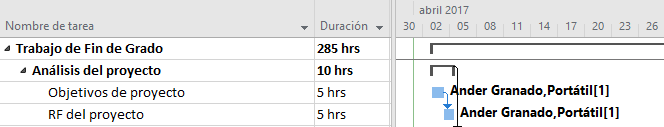
\includegraphics[width=1\textwidth]{TFG_GANTT_FASE_0}
	\caption{Cronograma de la fase inicial}
	\label{fig:gantt0}
\end{figure}

\begin{landscape}

\begin{figure}[H]
	\centering
	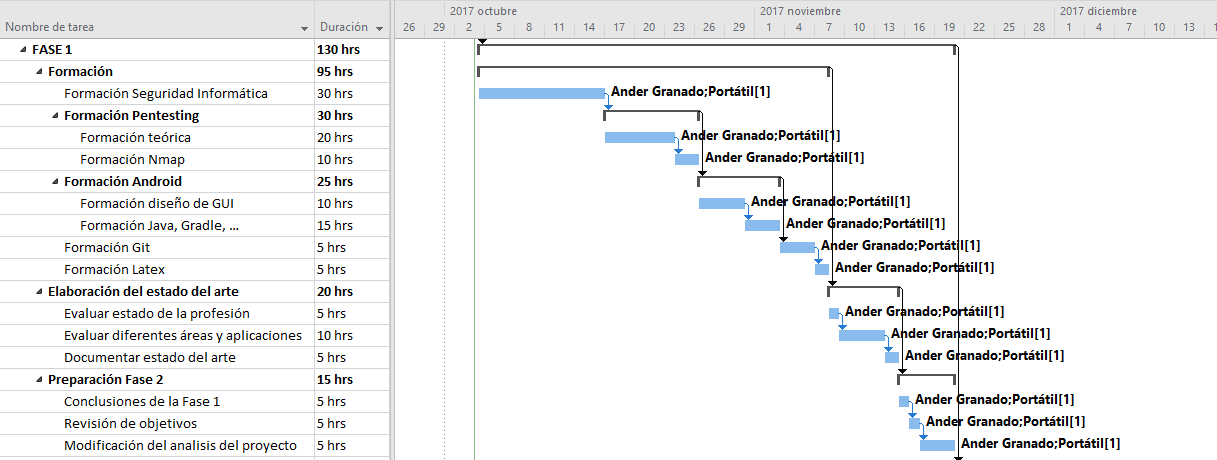
\includegraphics[height=210px]{TFG_GANTT_FASE_1}
	\caption{Cronograma de la Fase 1}
	\label{fig:gantt1}
\end{figure}

\begin{figure}[H]
	\centering
	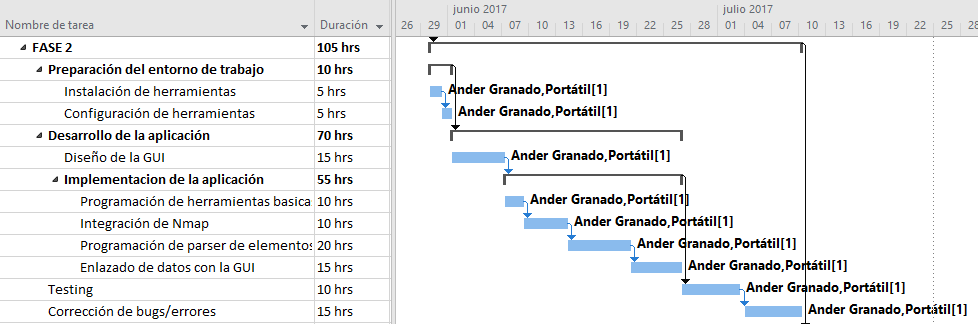
\includegraphics[height=160px]{TFG_GANTT_FASE_2}
	\caption{Cronograma de la Fase 2}
	\label{fig:gantt2}
\end{figure}

\end{landscape}

\begin{figure}[H]
	\centering
	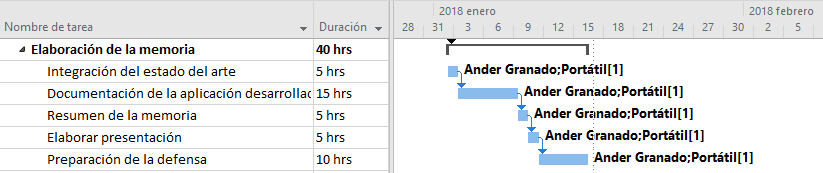
\includegraphics[width=1\textwidth]{TFG_GANTT_FASE_3}
	\caption{Cronograma de la elaboración de la memoria}
	\label{fig:gantt3}
\end{figure}



%------------------------------------------------------------------------------


\section{Gestión de costos}
A la hora de elaborar un análisis de costos, con el objetivo de obtener un presupuesto, primero es necesario identificar todos los recursos que influyen en ese presupuesto. Por una parte, tendremos los recursos de trabajo, es decir empelados, y por otra parte los recursos materiales, tanto de software como de hardware. En la \autoref{fig:recursos} se muestran tanto los recursos de trabajo como los recursos materiales de hardware.

\begin{figure}[H]
	\centering
	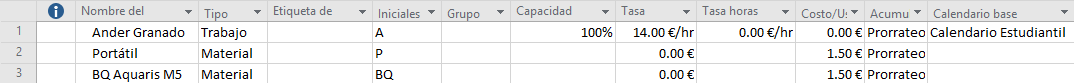
\includegraphics[width=1\textwidth]{TFG_RECURSOS}
	\caption{Recursos de trabajo y materiales}
	\label{fig:recursos}
\end{figure}

Por otra parte, en la \autoref{table:software} se muestra los recursos materiales de software utilizados.

\begin{table}[H]
	\centering
	\begin{tabular}{ |l|r| } 
		\hline
		\multicolumn{1}{|c|}{Concepto} & 
			\multicolumn{1}{|c|}{Coste} \\
		\hline
		Windows 10 		& 135,00 \euro \cite{precio-win10}		\\
		Project 2016 	& 1.369,00 \euro \cite{precio-project}	\\
		WBS Chart Pro 	& 187,50 \euro \cite{precio-wbs}		\\
		Ubuntu 16.04 	& 0,00 \euro							\\
		TeX Studio 		& 0,00 \euro							\\
		Android Studio 	& 0,00 \euro							\\
		Nmap 			& 0,00 \euro							\\
		Git 			& 0,00 \euro							\\
		GitHub 			& 0,00 \euro							\\
		\hline
	\end{tabular}
	\caption{Recursos materiales (software)}
	\label{table:software}
\end{table}


\subsection{Presupuesto}
El análisis de costes del proyecto se refleja en toda la información que aparecen entre la \autoref{table:recursos-trabajo} y la \autoref{table:total-presupuesto}. Para ello se tienen en cuanta varios puntos. El primero, se tiene en cuenta un salario base de 14 \euro/h, correspondiente un salario estándar de un analista programador.
Para los recursos materiales, se tiene en cuenta un costo por uso de 1,50 \euro. Estos costos por uso vienen dados por el gasto que generan debido al consumo energético, internet y otro tipo de gastos derivados de su utilización. Por otra parte se realiza una separación para los recursos de software, entre los que se incluye el propio Microsoft Project, software usado para la realización de todo el análisis de viabilidad y la gestión del proyecto.
Para el cálculo de las amortizaciones se considera un tiempo de amortización de 3 años, el cual traducido en horas vendría a ser 4800 horas ($3\ a\tilde{n}os\ *\ 200\ d\acute{i}as\ laborables\ *\ 8\ horas\ =\ 4800\ horas$).

\begin{table}[H]
	\centering
	\begin{tabular}{ |l|r| } 
		\hline
		\multicolumn{1}{|c|}{Concepto} & 
			\multicolumn{1}{|c|}{Coste} \\
		\hline
		Ander Granado & 14,00 \euro/h \\
		\hline
	\end{tabular}
	\caption{Recursos de trabajo}
	\label{table:recursos-trabajo}
\end{table}

\begin{table}[H]
	\centering
	\begin{tabular}{ |l|r| } 
		\hline
		\multicolumn{1}{|c|}{Concepto} & 
			\multicolumn{1}{|c|}{Coste} \\
		\hline
		Ordenador portátil 	& 700,00 \euro \\
		BQ Aquaris M5 		& 250,00 \euro \\
		\hline
	\end{tabular}
	\caption{Recursos materiales (hardware)}
	\label{table:recursos-materiales}
\end{table}

\begin{table}[H]
	\centering
	\begin{tabular}{ |l|r|r| } 
		\hline
		\multicolumn{1}{|c|}{Concepto} & 
			\multicolumn{1}{|c|}{Coste} & 
				\multicolumn{1}{|c|}{Número de licencias} \\
		\hline
		Windows 10 		& 135,00 \euro \cite{precio-win10} 		& 1 \\
		Project 2016 	& 1369,00 \euro \cite{precio-project} 	& 1 \\
		WBS Chart Pro 	& 187,50 \euro \cite{precio-wbs} 		& 1 \\
		Ubuntu 16.04 	& 0,00 \euro 							& 1 \\
		TeX Studio 		& 0,00 \euro							& 1 \\
		Android Studio 	& 0,00 \euro 							& 1 \\
		NMap 			& 0,00 \euro 							& 1 \\
		Git 			& 0,00 \euro 							& 1 \\
		GitHub 			& 0,00 \euro 							& 1 \\
		\hline
	\end{tabular}
	\caption{Recursos materiales (software)}
	\label{table:recursos-software}
\end{table}

\begin{table}[H]
	\centering
	\begin{tabular}{ |l|r|r|r|r|r| } 
		\hline
		\multicolumn{1}{|c|}{Concepto} & 
			\multicolumn{1}{|c|}{Trabajo (h)} & 
				\multicolumn{1}{|c|}{Trabajo horas extra} & 
					\multicolumn{1}{|c|}{Coste} & 
						\multicolumn{1}{|c|}{Coste horas extra} & 
							\multicolumn{1}{|c|}{Importe} \\
		\hline
		Ander Granado & 285 & 0 & 14,00 \euro/h & 0 & 4.044,00 \euro \\
		\hline
	\end{tabular}
	\caption{Costo de recursos de trabajo}
	\label{table:costo-recursos-trabajo}
\end{table}

\begin{table}[H]
	\centering
	\begin{tabular}{ |l|r|r|r| } 
		\hline
		\multicolumn{1}{|c|}{Concepto} & 
			\multicolumn{1}{|c|}{Unidades} & 
				\multicolumn{1}{|c|}{Coste} & 
					\multicolumn{1}{|c|}{Importe} \\
		\hline
		Ordenador portátil 	& 1 & 1,50 \euro/uso & 29 x 1,50 \euro \space= 43,50 \euro	\\
		BQ Aquaris M5 		& 1 & 1,50 \euro/uso & 7 x 1,50 \euro \space= 10,50 \euro	\\
		\hline
		\multicolumn{3}{|l}{TOTAL} & \multicolumn{1}{r|}{54,00 \euro} \\ 
		\hline
	\end{tabular}
	\caption{Costo de recursos materiales}
	\label{table:costo-recursos-materiales}
\end{table}

\begin{table}[H]
	\centering
	\begin{tabular}{ |l|r|r|r|r|r| } 
		\hline
		\multicolumn{1}{|c|}{Concepto} & 
			\multicolumn{1}{|c|}{Coste unitario} & 
				\multicolumn{1}{|c|}{T. de Amort.\tablefootnote{Tiempo de amortización}} & 
					\multicolumn{1}{|c|}{C.U.A.\tablefootnote{Coste unitario de amortización} (\euro)} & 
						\multicolumn{1}{|c|}{T. de uso} & 
							\multicolumn{1}{|c|}{Importe} \\
		\hline
		Ordenador portátil 		& 700,00 \euro 	& 4800 horas & 0,145833 \euro & 285 h	& 41,57 \euro	\\
		BQ Aquaris M5 			& 250,00 \euro 	& 4800 horas & 0,052083 \euro & 25 h	& 1,30 \euro	\\
		Windows 10 				& 135,00 \euro 	& 4800 horas & 0,028125 \euro & 180 h	& 5,06 \euro	\\
		M. Project 2016 	& 1.369,00 \euro & 4800 horas & 0,285208 \euro & 25 h	& 7,13 \euro 	\\
		WBS Chart Pro 			& 187,50 \euro 	& 4800 horas & 0,039062 \euro & 5 h		& 0,19 \euro	\\
		Ubuntu 16.04 			& 0,00 \euro 	& 4800 horas & 0,000000 \euro & 105 h	& 0,00 \euro	\\
		TeX Studio 				& 0,00 \euro 	& 4800 horas & 0,000000 \euro & 40 h	& 0,00 \euro	\\
		Android Studio 			& 0,00 \euro 	& 4800 horas & 0,000000 \euro & 105 h	& 0,00 \euro	\\
		NMap 					& 0,00 \euro 	& 4800 horas & 0,000000 \euro & 30 h	& 0,00 \euro	\\
		Git 					& 0,00 \euro 	& 4800 horas & 0,000000 \euro & 145 h	& 0,00 \euro	\\
		GitHub 					& 0,00 \euro 	& 4800 horas & 0,000000 \euro & 145 h	& 0,00 \euro	\\
		\hline
		\multicolumn{5}{|l}{TOTAL} & \multicolumn{1}{r|}{55,25 \euro} \\ 
		\hline
	\end{tabular}
	\caption{Amortizaciones de hardware y software}
	\label{table:amortizaciones}
\end{table}

\begin{table}[H]
	\centering
	\begin{tabular}{ |l|r| } 
		\hline
		\multicolumn{1}{|c|}{Concepto} & 
			\multicolumn{1}{|c|}{Importe} \\
		\hline
		Recursos de Trabajo (R.T.)	& 4.044,00 \euro	\\
		Recursos Materiales (R.M.)	& 54,00 \euro		\\
		Costo fijo					& 0,00 \euro		\\
		Amortizaciones				& 55,25 \euro		\\
		\hline
		SUMA						& 4.153,25 \euro	\\
		\hline
		Gastos generales (10\%)		& 415,32 \euro		\\
		Beneficio (15\%)			& 622,99 \euro		\\
		\hline
		SUBTOTAL					& 5.191,56 \euro	\\
		IVA (21\%)					& 1.090.23 \euro	\\
		\hline
		TOTAL						& 6281.79 \euro		\\
		\hline
	\end{tabular}
	\caption{Total presupuesto}
	\label{table:total-presupuesto}
\end{table}

Con esto se concluye que, tal como figura en la \autoref{table:total-presupuesto}, el coste del proyecto asciende a la cantidad de \textit{seis mil doscientos ochenta y cinco con setenta y nueve euros} (6281.79 \euro).

%------------------------------------------------------------------------------

\section{Gestión de riesgos}

En este apartado se identifican y analizan las diferentes amenazas que puedan llegar a impedir el correcto desarrollo del proyecto, haciendo que éste se retrase. Para ello primero se identifican los diferentes riesgos que pueden existir y se indica su peligrosidad. La peligrosidad es un valor cualitativo que indica en que medida puede afectar ese riesgo al proyecto.

Se han identificado los siguientes riesgos, los cuales se muestran en la \autoref{table:riesgos}.

\begin{table}[H]
	\centering
	\begin{tabular}{ |l|c| } 
		\hline
		\multicolumn{1}{|c|}{Riesgo} & 
		\multicolumn{1}{|c|}{Peligrosidad} \\
		\hline
			Pérdida de información										& Alta	\\
			Enfermedades												& Alta	\\
			Dificultades en la implementación de la aplicación			& Alta	\\
			Dedicación no exclusiva al trabajo							& Media	\\
			Averías o problemas técnicos con los recursos materiales	& Media	\\
			Cambios o ampliación de requisitos							& Media	\\
			Planificación muy optimista									& Media	\\
		\hline
	\end{tabular}
	\caption{Enumeración de riesgos del proyecto}
	\label{table:riesgos}
\end{table}


\subsection{Explicación y plan de contingencia}
Tras haber identificado los riesgos inherentes al proyecto en la \autoref{table:riesgos}, se hace mayor hincapié en los detalles de dicho riesgos, elaborando una descripción más detallada y analizando su probabilidad. La probabilidad de cada riesgo se muestra de manera cualitativa, ya que aportar un valor numérico concreto en este tipo de casos resulta bastante complicado. También, junto a lo mencionado, se añade para cada riesgo un plan de contingencia. El plan de contingencia consiste básicamente en aportar medidas para afrontar dicho riesgo, tanto preventivas (para antes de que ocurra) como correctoras (para en caso de ocurrir).

\riskframe
	{Pérdida de información}
	{Podría darse el caso de que parte de la información, como la memoria del proyecto, el estado del arte o el código de la aplicación se perdieran}
	{Baja}
	{Alta}
	{Uso de herramientas de control de versiones como Git junto a uso de herramientas cloud como GitHub o Dropbox}
	{Recuperación de la información mediante herramientas de análisis de unidades}

\riskframe
	{Enfermedades}
	{Podría suceder que el único recurso de trabajo contrajera una enfermedad o tuviera un accidente}
	{Baja}
	{Alta}
	{Ninguna}
	{Usar horas fuera del calendario para corregir el retraso en el proyecto}


\riskframe
	{Dificultades en la implementación de la aplicación}
	{Podría suceder que, durante la implementación de la aplicación, se dieran dificultades a nivel de programación a la hora de cumplir con los Requisitos Funcionales}
	{Media}
	{Alta}
	{Una formación sólida en las herramientas y tecnologías que se van a usar para el desarrollo de la aplicación}
	{Replantear las tareas posteriores y dedicar un esfuerzo extra para el aprendizaje y refuerzo de las herramientas usadas}

\riskframe
	{Dedicación no exclusiva al trabajo}
	{Podría suceder que, debido a exámenes u otros asuntos personales, el desarrollador no pudiera aportar toda la dedicación que requiere el proyecto}
	{Media}
	{Media}
	{No previsible}
	{Cambiar calendario de trabajo aumentando las horas para subsanar los retrasos producidos por dicho riesgo}

\riskframe
	{Averías o problemas técnicos con los recursos materiales}
	{Podría darse el caso de que alguno de los recursos materiales de hardware, como el ordenador o el teléfono móvil, sufran algún tipo de avería}
	{Baja}
	{Media}
	{No previsible}
	{Uso de otros dispositivos para continuar con el desarrollo del proyecto, adquiridos mediante compra o préstamo}

\riskframe
	{Cambios o ampliación de requisitos}
	{Podría darse el caso en el que, tras la conclusión de la Fase 1, se cambiarán Requisitos Funcionales de la aplicación a desarrollar o se añadirán nuevos Requisitos Funcionales}
	{Media - Alta}
	{Media}
	{Revisión constante de los Requisitos Funcionales durante todas las fases del proyecto para minimizar el impacto que pueda causar los cambios en ellos}
	{Adaptar el calendario las tareas posteriores y el calendario de trabajo actual}

\riskframe
	{Planificación muy optimista}
	{Puede darse el caso de que la planificación elaborada para el proyecto sea demasiado optimista y no haya tenido en cuenta ciertos aspectos más concretos del desarrollo del proyecto}
	{Media}
	{Media}
	{No previsible}
	{Adaptar, y en caso de que fuera necesario retrasar, la fecha final del proyecto para dar cabida en la planificación toda  esa duración extra no prevista}